\documentclass[main.tex]{subfiles}
% 标架与参考系
\begin{document}
接下来为了讨论的方便,我们对时间段$\Upsilon$下的给定的运动过程$\chi$规定记法$\chi_t:B\rightarrow\pazocal{W},$
\[\chi_t\left(X\right)=\chi\left(X,t\right),\quad\forall X\in B,t\in\Upsilon\]

设一名观察者观察一个物体$B$在时间段$\Upsilon$内的运动过程$\chi$,这名观察者要确定的是物体$B$相对于他选择的参考标架$\left(\mathcal{E},\phi\right)$的运动。在同一时段$\Upsilon$内,定义映射$\kappa:B\times\Upsilon\rightarrow\mathcal{E},$
\[\kappa\left(X,t\right)=\kappa_t\left(X\right)=\phi_t^{-1}\circ\chi_t\left(X\right),\forall X\in B, t\in\Upsilon\]
则$\kappa$在形式上定义了“物体$B$在物体$\mathcal{E}$内的运动过程”,而事实上$\mathcal{E}$是这名观察者选择的参考标架的欧几里得空间。我们称$\kappa$为\emph{物体$B$相对于参考标架$\left(\mathcal{E},\phi\right)$的由$\chi$确定的运动},它由物体$B$的客观运动过程$\chi$和参考标架本身的客观运动过程$\phi$共同确定。任一观察者在不与其他观察者交流的情况下,只能感知相对运动$\kappa$。

\begin{figure}[ht]
    \centering
    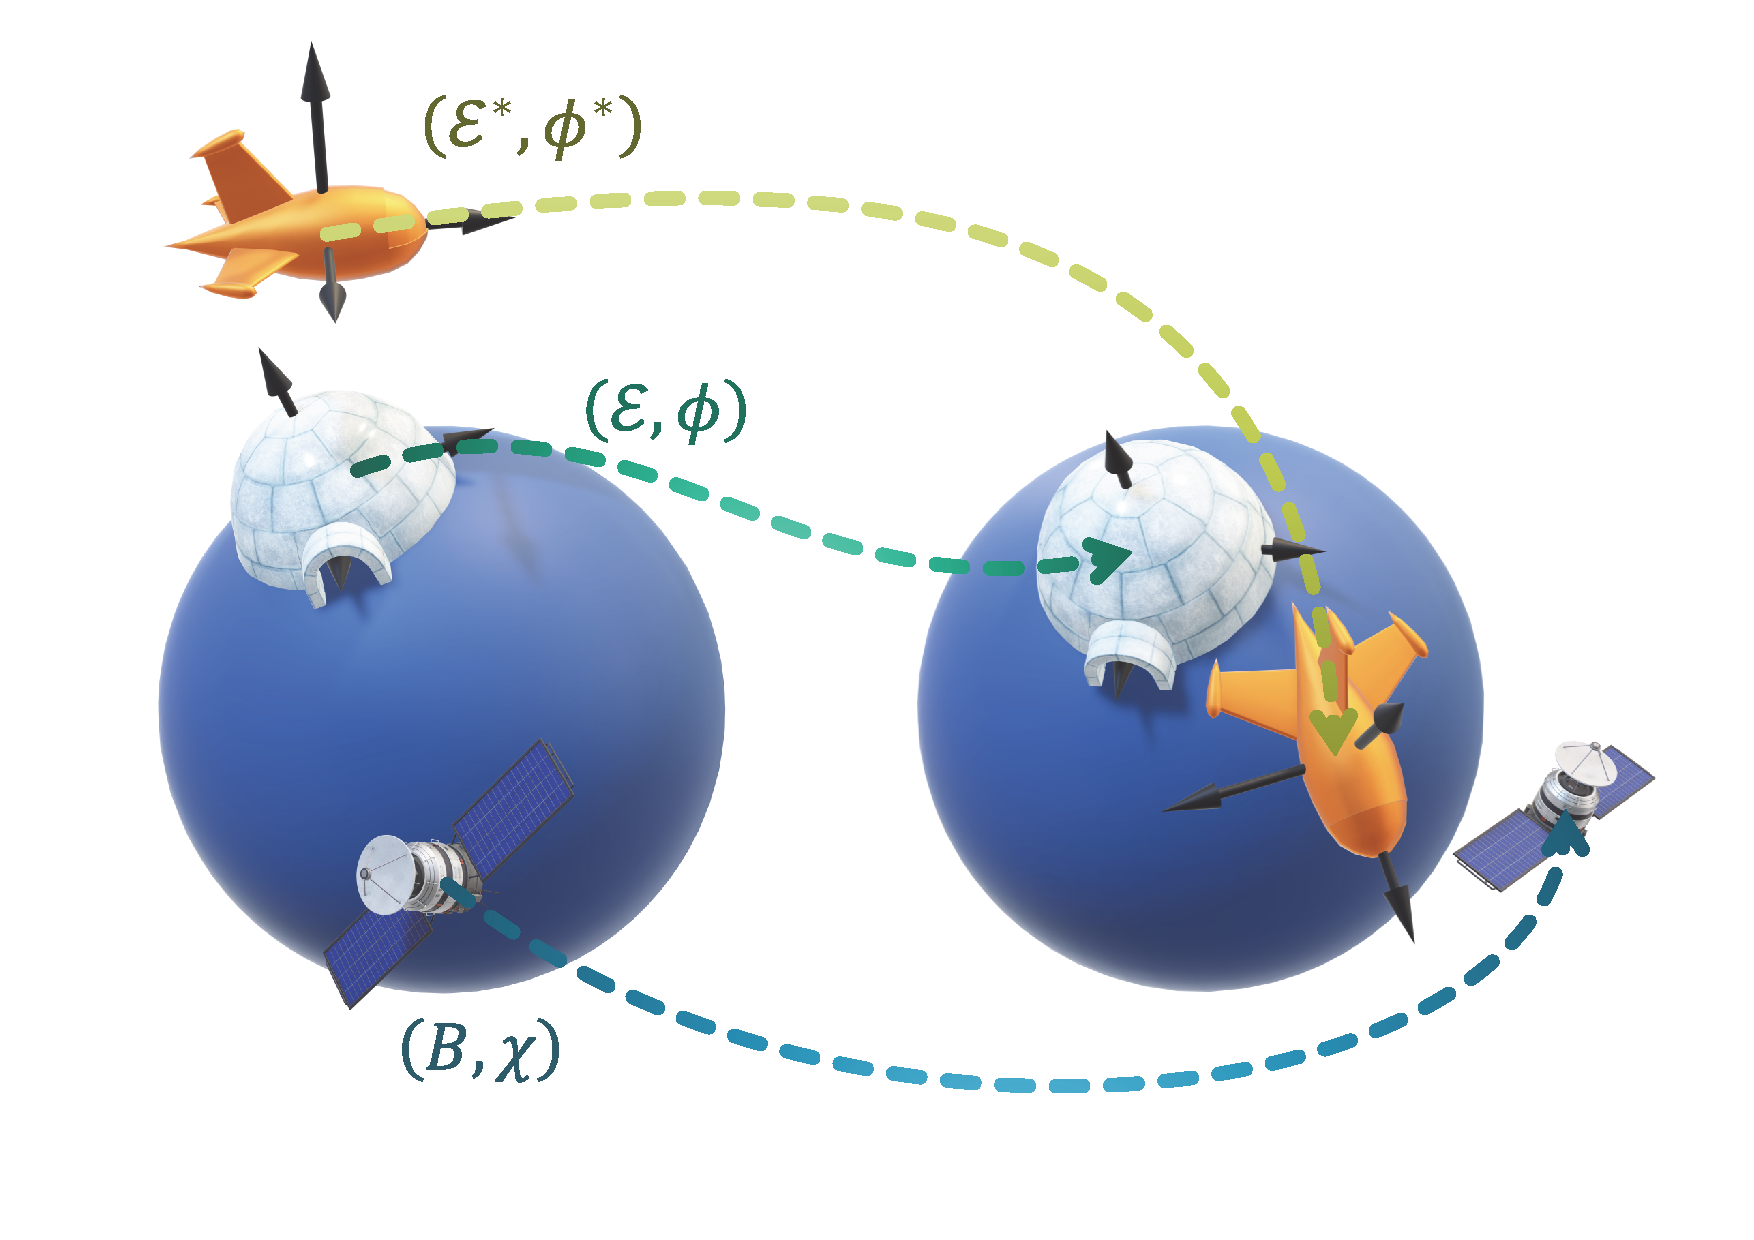
\includegraphics[width=0.5\textwidth]{images/III.5.3.pdf}
    \caption{不同观察者在各自的标架$\left(\mathcal{E},\phi\right)$、$\left(\mathcal{E}^*,\phi^*\right)$下观察同一物体$B$的运动过程$\chi$。尽管刚体系$\mathcal{E}$和$\mathcal{E}^*$各自也有运动$\phi$、$\phi^*$,但每个观察者都只能感知到$B$相对各自标架的运动$\kappa$、$\kappa^*$(未标出)。观察者之间通过交流,也只能额外了解到两标架之间的相对运动$\phi^{*-1}\circ\phi$(未标出)。}
    \label{fig:III.5.3}
\end{figure}

假设有两名观察者分别选择了标架$\left(\mathcal{E},\phi\right)$和$\left(\mathcal{E}^*,\phi^*\right)$,$d$、$d^*$是按前面所述由$\phi$、$\phi^*$定义的度量。这两名观察者观察同一物体$B$在时间段$\Upsilon$内的一个运动过程$\chi$,将各自感知为$B$相对标架$\left(\mathcal{E},\phi\right)$、$\left(\mathcal{E}^*,\phi^*\right)$的运动过程$\kappa$和$\kappa^*$(可结合图\ref{fig:III.5.3}来理解)。按照前面介绍过的定义,
\[\kappa_t=\phi_t^{-1}\circ\chi_t,\quad\kappa_t^*=\phi_t^{*-1}\circ \chi_t,\quad\forall t\in\Upsilon\]
故有
\[\kappa_t^*=\left(\phi_t^{*-1}\circ\phi_t\right)\circ\kappa_t,\quad\forall t\in\Upsilon\]
也就是说,两名观察者任一时刻所感知到的相对运动之间,只相差$\phi_t^{*-1}\circ\phi_t$,而这是$\mathcal{E}$作为一个刚体系相对于标架$\left(\mathcal{E}^*,\phi^*\right)$的由$\phi$确定的运动。两名观察者通过交流,也只能感受到这一标架间的相对运动,而无法单独感知到$\phi$或$\phi^*$。这一标架间的相对运动$\phi_t^{*-1}\circ\phi_t$是标架变换的讨论重点。

留意到,在时间段$\Upsilon$内的每一时刻$t$下,$\left(t,\delta\right)$、$\left(\mathcal{E},d\right)$、$\left(\mathcal{E}^*,d^*\right)$是三个欧几里得度量空间,$\phi_t$、$\phi_t^*$分别是由$\mathcal{E}$到$t$、$\mathcal{E}^*$到$t$的等距变换,故复合映射$\phi_t^{*-1}\circ\phi_t$是由$\mathcal{E}$到$\mathcal{E}^*$的、依赖时刻$t$的等距变换。在此我们可以利用等距变换的表示定理(定理\ref{thm:II.3.2})写出复合映射$\phi_t^{*-1}\circ\phi_t$的形式。具体地,物体$B$在时间段$\Upsilon$内的运动过程$\chi$中,时刻$t\in\Upsilon$下,物质点$P_X\in B$在时刻$t$下分别对应于欧几里得空间$\mathcal{E}$、$\mathcal{E}^*$中的点$X\left(t\right)$、$X^*\left(t\right)$,则有
\[X\left(t\right)=\kappa_t\left(P_X\right),\quad X^*\left(t\right)=\kappa_t^*\left(P_X\right),\quad t\in\Upsilon\]
其中$\kappa$、$\kappa^*$分别是物体$B$在时间段$\Upsilon$内相对于标架$\left(\mathcal{E},\phi\right)$、$\left(\mathcal{E}^*,\phi^*\right)$的运动。由之前介绍过的定义我们有
\[X^*\left(t\right)=\phi_t^{*-1}\circ\phi_t\left(X\left(t\right)\right),\quad\forall t\in\Upsilon\]
上式说明,两个观察者在各自的参考标架下,对同一物理事件的空间定位,相差一个等距变换。由定理\ref{thm:II.3.2},再任意给定一物质点$P_{X_0}\in B$,就有
\[X^*\left(t\right)=X_0^*\left(t\right)+\mathbf{Q}_t\left(X\left(t\right)-X_0\left(t\right)\right)\]
其中
\[X_0\left(t\right)=\kappa_t\left(P_{X_0}\right),\quad X_0^*\left(t\right)=\kappa_t^*\left(P_{X_0}\right),\quad t\in\Upsilon\]
注意到,由于每一时刻$t$下的等距变换$\phi_t^{*-1}\circ\phi_t$是不同的等距变换,因此上式中的正交算符$\mathbf{Q}_t$依赖$t$而变化。另外,由\S\ref{sec:II.3.4}最后的讨论,$\mathrm{det}\mathbf{Q}_t\equiv 1$。

给定一个欧几里得空间,也就同时给定了它的平移空间和一个基本直角坐标系。因此每个欧几里得空间点集里的点,唯一对应于它在这一基本直角坐标系下的位置向量,也唯一对应于一个有序实数三元组。故上式的成立同时意味着下式的成立
\[\mathbf{r}_X^*\left(t\right)=\mathbf{r}_{X_0}^*\left(t\right)+\mathbf{Q}_t\left(\mathbf{r}_X\left(t\right)-\mathbf{r}_{X_0}\left(t\right)\right)\]
其中$\mathbf{r}^*_{X_0}\left(t\right)=X_0^*\left(t\right)-O\left(t\right)\cdots\in\mathbb{R}^3$等都是相应的点在其所属的欧几里得空间中的基本直角坐标。

在时刻空间$\pazocal{T}$中,只要选定一个时刻$t_0$作为\emph{时间原点(time origin)},那么由之前关于时刻空间的讨论,任一时刻$t$都唯一对应$\mathbb{R}$中的一个实数$s=t-t_0$,任一实数$s$总有唯一一个时刻$t$满足$s=t-t_0$。也就是说,只要选定了时间原点$t_0$,那么时刻空间$\pazocal{T}$的元素就与实数一一对应。
假定两个观察者选定不同的时刻$t_0$、$t_0^*\in\pazocal{T}$作为原点时刻,那么他们会相应使用不同的实数$s$、$s^*\in\mathbb{R}$来标记同一时刻$t\in\pazocal{T}$。正如$\mathbf{r}^*_X$与$\mathbf{r}_X$的关系那样,$s$与$s^*$的换算关系也是被时空结构的定义确定的。为了得出这个关系,我们将一名观察者把一个时刻对应成一个实数的映射记为双射$T:\pazocal{T}\rightarrow\mathbb{R}$。两个不同观察者分别采用映射$T$、$T^*$把同一时刻$t\in\pazocal{T}$记作不同的实数。易验$T,T^*$满足
\[\left|T\left(t_1\right)-T\left(t_2\right)\right|=\left|T^*\left(t_1\right)-T^*\left(t_2\right)\right|=\left|t_1-t_2\right|,\quad\forall t_1,t_2\in\pazocal{T}\]
因此$T$、$T^*$都是度量空间$\left(\pazocal{T},\left|\overline{\tau}\right|\right)$的上的等距变换。那么复合映射$T^{*-1}\circ T$就是$\mathbb{R}$上的一个等距变换。由等距变换的表示定理,对任意$s\in\mathbb{R}$,
\[s^*=s_0^*+\left(s-s_0\right)\]
其中$s_0^*=T^{*-1}\circ T\left(s_0\right)$;在$\mathbb{R}$上,正交算符就是$\pm 1$;行列式为1的正交算符就是1。上式又可整理成
\[s^*=s+a\]
其中由$T$、$T^*$的等距变换事实可知$a=s_0^*-s_0=t_0^*-t_0$是只依赖时间原点选择的常实数。。

把以上分析的结果进行总结:两名观察者$O$、$O^*$对同一物体的运动过程进行观测,在各自选定的时间原点$t_0$、$t_0^*$和参考标架$\left(\mathcal{E},\phi\right)$、$\left(\mathcal{E}^*,\phi^*\right)$下,$O$用于描述时刻$t\in\pazocal{T}$下的两个事件$e,e_0\in\pazocal{W}$的实数组$\left(s,\mathbf{r}\left(s\right)\right)$、$\left(s,\mathbf{r}_0\left(s\right)\right)$和$O^*$用于描述同一时刻$t$的相同两个事件$e,e_0$的实数$\left(s^*,\mathbf{r}^*\left(s^*\right)\right)$、$\left(s^*,\mathbf{r}^*_0\left(s^*\right)\right)$之间存在以下换算关系——
\begin{align*}
    s^*                          & =s+a                                                                                                         \\
    \mathbf{r}^*\left(s^*\right) & =\mathbf{r}_0^*\left(s^*\right)+\mathbf{Q}_t\left(\mathbf{r}\left(s\right)-\mathbf{r}_0\left(s\right)\right)
\end{align*}
其中$a=t_0^*-t_0$是常实数,$\mathbf{Q}_t$是$\mathbb{R}^3$上的正交变换(即一个$3\times 3$实正交矩阵)且$\mathrm{det}\mathbf{Q}_t\equiv 1$。我们称上述变换为一个\emph{标架变换(change of frame)}。

上列的标架变换关系式,是由新经典时空的定义和参考标架的定义推导得出的数学结果。从它的形式上看,不同的参考标架之间,没有“钟慢效应”和“尺缩效应”,这亦是新经典时空结构本身蕴含的性质。回顾新经典时空的定义可以看到,同时性的定义方式是绝对的,欧几里得度量的定义方式也是绝对的,故有此结果。

我们对同一物理事件的观测,可能得到依赖这一事件的不同物理量。在选定了标架之后,这样的物理量是依赖时间和空间的场函数,而它的函数值可以是标量、向量和线性算符。具体地,在两个标架$\left(\mathcal{E},\phi\right)$、$\left(\mathcal{E}^*,\phi^*\right)$下,对同一物理事件观测得到的标量、向量和线性算符场函数分别记为:
\begin{align*}
    \alpha,\alpha^*:\mathbb{R}^{1+3}\supset D\rightarrow\mathbb{R},\quad                                   & \alpha\left(t,\mathbf{r}\right),\quad      \alpha^*\left(t^*,\mathbf{r}^*\right)     \\
    \mathbf{a},\mathbf{a}^*:\mathbb{R}^{1+3}\supset D\rightarrow\mathbb{R}^3,\quad                         & \mathbf{a}\left(t,\mathbf{r}\right),\quad  \mathbf{a}^*\left(t^*,\mathbf{r}^*\right) \\
    \mathbf{A},\mathbf{A}^*:\mathbb{R}^{1+3}\supset D\rightarrow\mathcal{L}\left(\mathbb{R}^3\right),\quad & \mathbf{A}\left(t,\mathbf{r}\right),\quad  \mathbf{A}^*\left(t^*,\mathbf{r}^*\right)
\end{align*}
其中$t,t^*\in\mathbb{R}$,$\mathbf{r},\mathbf{r}^*\in\mathbb{R}^3$。设$\mathbf{Q}_t$是由$\left(\mathcal{E},\phi\right)$到$\left(\mathcal{E}^*,\phi^*\right)$的标架变换的正交算符。若对\emph{任意}两标架$\left(\mathcal{E},\phi\right)$、$\left(\mathcal{E}^*,\phi^*\right)$,上述物理量都满足
\begin{align*}
    \alpha^*\left(t^*,\mathbf{r}^*\right)     & =\alpha\left(t,\mathbf{r}\right)                                       \\
    \mathbf{a}^*\left(t^*,\mathbf{r}^*\right) & =\mathbf{Q}_t\mathbf{a}\left(t,\mathbf{r}\right)                       \\
    \mathbf{A}^*\left(t^*,\mathbf{r}^*\right) & =\mathbf{Q}_t\mathbf{A}\left(t,\mathbf{r}\right)\mathbf{Q}_t^\intercal
\end{align*}
则称这些物理量具有\emph{标架变换下的不变性(invariance under change of frames)}。

为什么要这样定义呢?客观的标量值物理性质,本应不依赖观察的参考标架。设某时刻下空间某处有某偶极矩$\boldsymbol{\mu}$,这是一个客观现象。在不同的参考标架下,这一偶极矩将被“画”在不同坐标系下的欧几里得空间当中,各具有一组坐标$\mathbf{u},\mathbf{u}^*\in\mathbb{R}^3$。在同一时刻下,两个标架的欧几里得空间$\mathcal{E}$和$\mathcal{E}^*$的差别,可视为同一欧几里得空间内的两个直角坐标系。那么,同一向量在这两种情况之间的差别,将只相差一个由该时刻下这两个直角坐标系决定的正交矩阵$\mathbf{Q}_t$作为过渡矩阵的坐标变换公式,即$\mathbf{u}^*=\mathbf{Q}_t\mathbf{u}$。同理,线性变换值的物理量,在每一时刻下的两个标架下的坐标矩阵之间也相差一个由这两个标架确定的正交矩阵$\mathbf{Q}_t$作为过渡矩阵的坐标变换公式,即$\mathbf{A}^*=\mathbf{Q}_t\mathbf{A}\mathbf{Q}_t^\intercal$。可见,标架变换下的不变性定义,道出的是具有客观的物理量应该满足的条件。但是,物理量的定义及其依附的经验规律(方程)是有无限可能的,并不一定都满足标架变换不变性。

但至少,同一观察者,对同一物理量的观测结果,必须具有不依赖坐标系选择的客观性。这里包括曲线坐标系选择。然而,标量、向量和线性算符物理量及其微积分在曲线坐标变换下的数学形式遵守一套系统的理论——\emph{张量分析(tensor analysis)}。当我们说“标量、向量和线性算符是都是张量”时,我们实际上是主张赋予作为代数结构的标量、向量和线性算符以曲线坐标变换的理论支撑。只要注意按照曲线坐标系理论来处理物理量的坐标变换,就能使物理量满足不依赖坐标系选择的客观性。这件事在一般的教材中又叫做“用张量来表示物理量”。这是之所以要求用张量来描述流变学的本构关系的根本原因。
\end{document}